\documentclass[tikz]{standalone}
\usetikzlibrary{positioning}
% newcommands.tex

\newcommand{\enq}{\texttt{enq}}
\newcommand{\deq}{\texttt{deq}}
\newcommand{\pput}{\texttt{PUT}}
\newcommand{\get}{\texttt{GET}}
\newcommand{\vs}{\texttt{vis}}
\newcommand{\so}{\texttt{so}}
\newcommand{\arb}{\texttt{ar}}
\newcommand{\rf}{\texttt{rf}}

% example
\newcommand{\po}[2]{\draw [->, thick] (#1) to node[above] {\Large{\so}} (#2);}
\newcommand{\pva}[2]{\draw [->, thick] (#1) to node[above] {$\Large{\so},\Large{\vs},\Large{\arb}$} (#2);}
\newcommand{\pbva}[2]{\draw [->, thick] (#1) to node[above] {$\Large{\so}$} node[below] {$\Large{\vs},\Large{\arb}$} (#2);}
\newcommand{\pv}[2]{\draw [->, thick] (#1) to node[above] {\Large{\so}} node[below] {\Large{\vs}} (#2);}
\newcommand{\evis}[2]{\draw [->, thick] (#1) to node[above, sloped, near end] {\Large{\vs}} (#2);}
\newcommand{\mvis}[2]{\draw [->, thick] (#1) to node[above, sloped] {\Large{\vs}} (#2);}
\newcommand{\ar}[2]{\draw [->, thick, allow upside down] (#1) to node[above, sloped] {\Large{\arb}} (#2);}
\newcommand{\va}[2]{\draw [->, thick, allow upside down] (#1) to node[above, sloped] {$\Large{\vs},\Large{\arb}$} (#2);}
\newcommand{\vab}[2]{\draw [->, thick, allow upside down] (#1) to node[below, sloped, near end] {$\Large{\vs},\Large{\arb}$} (#2);}
\newcommand{\vae}[2]{\draw [->, thick, allow upside down] (#1) to node[above, sloped, near end] {$\Large{\vs},\Large{\arb}$} (#2);}
\newcommand{\vas}[2]{\draw [->, thick, allow upside down] (#1) to node[sloped, near start, above] {$\Large{\vs},\Large{\arb}$} (#2);}

% serialization
\newcommand{\scc}[2]{\draw [->, very thick] (#1) to (#2);}
\newcommand{\rva}[2]{\draw [->, thick, allow upside down] (#1) to node[above, sloped] {$\Large{\rf},\Large{\vs},\Large{\arb}$} (#2);}
\newcommand{\rvb}[2]{\draw [->, thick, allow upside down] (#1) to node[below, sloped] {$\Large{\rf},\Large{\vs},\Large{\arb}$} (#2);}


%\renewcommand{\va}[2]{\draw [->, thick, allow upside down] (#1) to node[above, sloped] {$\Large{\vs}$} node[below, sloped] {$\Large{\arb}$} (#2);}
%\renewcommand{\va}[2]{\draw [->, thick] (#1) to node[above, pos=0.4] {$\Large{\vs},\Large{\arb}$} (#2);}
\renewcommand{\va}[2]{\draw [->, thick] (#1) to (#2);}

\begin{document}
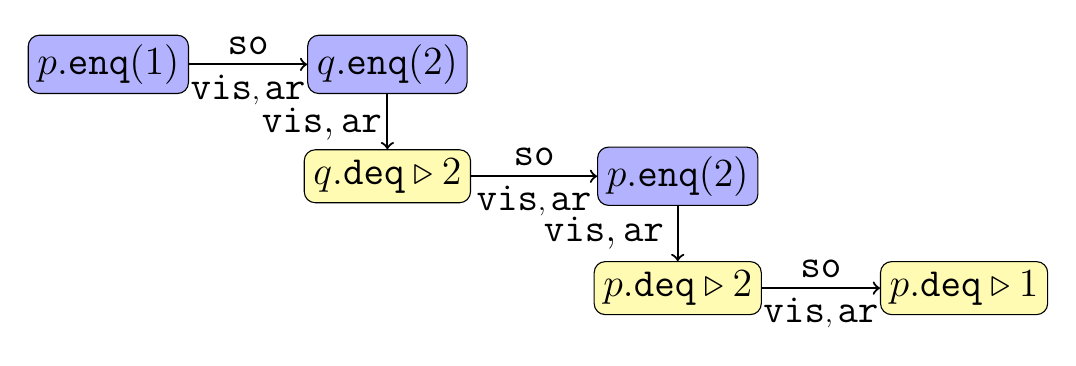
\begin{tikzpicture}
\tikzset{
  enq-op/.style = {rectangle, rounded corners, fill = blue!30, draw, font = \Large},
  deq-op/.style = {rectangle, rounded corners, fill = yellow!30, draw, font = \Large},
  process/.style = {font = \huge},
  vis/.style = {rectangle, font = \Large}
}

  %\node (p1) [process] {$p_1:$};
  %\node (p1-enq1) [enq-op, right = 0.5cm of p1] {$p.\enq(1)$};
  \node (p1-enq1) [enq-op] {$p.\enq(1)$};
  \node (p1-enq2) [enq-op, right = 1.5cm of p1-enq1] {$q.\enq(2)$};

  %\node (p2) [process, below = 0.7cm of p1] {$p_2:$};
  \node (p2-deq2) [deq-op, below = 0.7cm of p1-enq2] {$q.\deq\triangleright2$};
  \node (p2-enq2) [enq-op, right = 1.6 of p2-deq2] {$p.\enq(2)$};

  %\node (p3) [process, below = 0.7cm of p2] {$p_3:$};
  \node (p3-deq2) [deq-op, below = 0.7cm of p2-enq2] {$p.\deq\triangleright2$};
  \node (p3-deq1) [deq-op, right = 1.5cm of p3-deq2] {$p.\deq\triangleright1$};

  \pbva{p1-enq1}{p1-enq2};
  \pbva{p2-deq2}{p2-enq2};
  \pbva{p3-deq2}{p3-deq1};

  \node [vis, below right = 0.05cm and 0.8cm of p1-enq1] {$\vs,\arb$};
  \node [vis, below right = 0.05cm and 0.8cm of p2-deq2] {$\vs,\arb$};

  \va{p1-enq2}{p2-deq2};
  \va{p2-enq2}{p3-deq2};

\end{tikzpicture}
\end{document}
